%% Copyright (c) 2015-2020, RTE (http://www.rte-france.com)
%% See AUTHORS.txt
%% All rights reserved.
%% This Source Code Form is subject to the terms of the Mozilla Public
%% License, v. 2.0. If a copy of the MPL was not distributed with this
%% file, you can obtain one at http://mozilla.org/MPL/2.0/.
%% SPDX-License-Identifier: MPL-2.0
%%
%% This file is part of Dynawo, an hybrid C++/Modelica open source time domain simulation tool for power systems.

\documentclass[a4paper, 12pt]{report}

%%  Copyright (c) 2015-2019, RTE (http://www.rte-france.com)
%%  See AUTHORS.txt
%%  All rights reserved.
%%  This Source Code Form is subject to the terms of the Mozilla Public
%%  License, v. 2.0. If a copy of the MPL was not distributed with this
%%  file, you can obtain one at http://mozilla.org/MPL/2.0/.
%%  SPDX-License-Identifier: MPL-2.0
%%
%%  This file is part of Dynawo, an hybrid C++/Modelica open source time domain
%%  simulation tool for power systems.


%%%%%%%%%%%%%%%%%%%%%%%%%%%%%%%%%%%%%%%%%%%
% Define text and document settings
%%%%%%%%%%%%%%%%%%%%%%%%%%%%%%%%%%%%%%%%%%%

\usepackage{lmodern} % Latin Modern fam­ily of fonts
\usepackage[english]{babel} % English

% Specify encoding
\usepackage[utf8]{inputenc} % Input
\usepackage[T1]{fontenc} % Output

% Document structure setup
\usepackage{titlesec} % To change chapter format
\setcounter{tocdepth}{3} % Add subsubsection in Content
\setcounter{secnumdepth}{3} % Add numbering for subsubsection
\setlength{\parindent}{0pt} % No paragraph indentation

% Avoid numbering starting at each chapter for figures
\usepackage{chngcntr}
\counterwithout{figure}{chapter}

% Change title format for chapter
\titleformat{\chapter}{\Huge\bf}{\thechapter}{20pt}{\Huge\bf}

% To add links on page number in Content and hide red rectangle on links
\usepackage[hidelinks, linktoc=all]{hyperref}
\usepackage[nottoc]{tocbibind} % To add biblio in table of content
\usepackage{textcomp} % For single quote
\usepackage{url} % Allow linebreaks in \url command
\usepackage{listings} % To add code samples

% Define typography
\usepackage{xspace}
\usepackage{dirtree}
\newcommand{\Dynawo}[0]{Dyna$\omega$o\xspace}

% Default listings parameters
\lstset
{
  aboveskip={1\baselineskip}, % A bit of space above
  backgroundcolor=\color{shadecolor}, % Choose the background color
  basicstyle={\ttfamily\footnotesize}, % Use font and smaller size \small \footnotesize
  breakatwhitespace=true, % Sets if automatic breaks should only happen at whitespace
  breaklines=true, % Sets automatic line breaking
  columns=fixed, % Nice spacing -> fixed / flexible
  mathescape=false, % Escape to latex false
  numbers=left, % Where to put the line-numbers
  numberstyle=\tiny\color{gray}, % The style that is used for the line-numbers
  showstringspaces=false, % Do not emphasize spaces in strings
  tabsize=4, % Number of spaces of a TAB
  texcl=false, % Activates or deactivates LaTeX comment lines
  upquote=true % Upright quotes
}

%%%%%%%%%%%%%%%%%%%%%%%%%%%%%%%%%%%%%%%%%%%
% Define plots settings
%%%%%%%%%%%%%%%%%%%%%%%%%%%%%%%%%%%%%%%%%%%

% Macro pack­age for cre­at­ing graph­ics
\usepackage{tikz}
\usepackage{subfigure}
\usepackage{float}

% Draws func­tion plots (based on pgf/tikz)
\usepackage{pgfplots}
\pgfplotsset{enlarge x limits=false, xlabel={\begin{small}$time$ (s)\end{small}}, height=0.6\textwidth, width=1\textwidth}
\pgfplotstableset{col sep=semicolon}

% Define colors
\usepackage{color}
\definecolor{blue}{rgb}{.3,.5,1}
\definecolor{deepblue}{rgb}{0,0,1}
\definecolor{darkblue}{rgb}{0,0,.4}
\definecolor{red}{rgb}{1,0,0}
\definecolor{darkred}{rgb}{.56,0,0}
\definecolor{pink}{rgb}{.933,0,.933}
\definecolor{purple}{rgb}{0.58,0,0.82}
\definecolor{green}{rgb}{0.133,0.545,0.133}
\definecolor{darkgreen}{rgb}{0,.4,0}
\definecolor{gray}{rgb}{.3,.3,.3}
\definecolor{darkgray}{rgb}{.2,.2,.2}
\definecolor{shadecolor}{gray}{0.925}

%%%%%%%%%%%%%%%%%%%%%%%%%%%%%%%%%%%%%%%%%%%
% Define blocks for simple network drawings
%%%%%%%%%%%%%%%%%%%%%%%%%%%%%%%%%%%%%%%%%%%

% Define blocks for newtorks drawings
\usepackage{amsmath} % Add math­e­mat­i­cal fea­tures
\usepackage{schemabloc} % Add block diagram library (french one)

%% Define infinite bus
\tikzset{infinite bus/.pic={
  code={
  \draw (0,0) circle (2) node[inner sep=0, outer sep=0] {{$\infty$}};
  \draw (2,0) --++ (2,0);
  }
  }
}

%% Define transformer
\tikzset{transfo/.pic={
  code={
  \draw (0,0) circle (2);
  \draw (2,0) circle (2);
  \draw (4,0) --++ (4,0);
  \draw (-2,0) --++ (-4,0);
  }
  }
}

%% Define generator
\tikzset{generator/.pic={
  code={
    \draw (0,0) circle (2);
    \draw (0,0) arc (0:180:0.5);
    \draw (0,0) arc (180:360:0.5);
    \draw (-2,0) --++ (-2,0);
  }
  }
}

%% Define generator controls
\tikzset{VR/.pic={
  code={
  \draw (0,0) circle (2) node[inner sep=0, outer sep=0] {{VR}};
  }
  }
}

%% Define SVarC
\tikzset{SVarC/.pic={
  code={
  \draw (0,0) circle (4) node[inner sep=0, outer sep=0] {{SVarC}};
  }
  }
}


\begin{document}

\chapter{IEEE14}

The IEEE 14-bus system is a standard test case in the power system community. It represents a simple approximation of the American Electric Power system (in the U.S. Midwest) as it was in the early 1960s. The data were provided by Iraj Dabbagchi of AEP and converted into the IEEE Common Data Format by Rich Christie at the University of Washington in August 1993.

% Generic description of the non regression test
% List of scenarios
\section{Test case description}

The IEEE 14-bus test case system has 14 buses, 5 generators (three of them being synchronous compensators used only for reactive support), 1 shunt, 3 transformers, 16 lines and 11 loads.\\
There are two voltage levels in the test case: 69 kV and 13.8 kV. The lower part of the system, with generators 1, 2 and 3, corresponds to the 69 kV network, whereas the upper part is the 13.8 kV network.

\begin{figure}[H]
  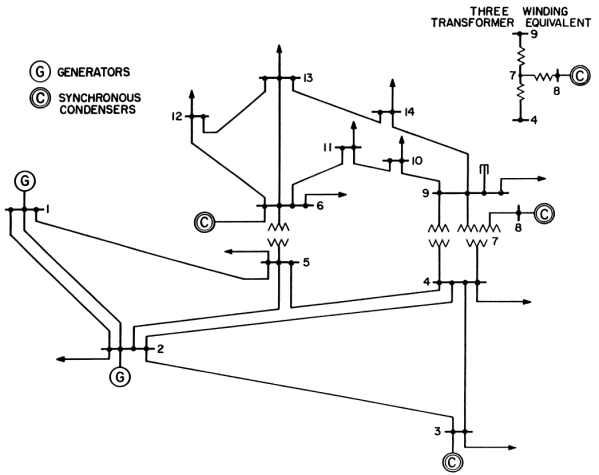
\includegraphics[width=\textwidth]{Single-line-diagram-of-IEEE-14-bus-system.png}
  \caption{IEEE 14 bus system diagram}
\end{figure}

\subsection{Initial Conditions}

The reference angle for the load flow is set at bus n°1. \\

Here are the initial conditions for each generator.

\begin{center}
\begin{tabular}{|c|c|c|c|c|}
  \hline
  Generator & P (MW) & Q (Mvar) & U (kV) & $\Theta$ (°) \\
  \hline
  1 & 232.39 & -16.55 & 73.14 & 0.00\\
  2 & 40.00 & 43.56 & 72.11 & -4.98\\
  3 & 0.00 & 25.07 & 69.69 & -12.73\\
  6 & 0.00 & 12.73 & 14.77 & -14.22\\
  8 & 0.00 & 17.62 & 15.04 & -13.36\\
  \hline
\end{tabular}
\end{center}

\subsection{Models}

\subsubsection{Synchronous Machines}

The generators are modelled using the GeneratorPVSignalN model. This model is used for the calculation of steady states after an event. All machines participate in the frequency regulation depending on their nominal active power (although the frequency is not explicitly modelled in this model). For each generator, the active power is indeed equal to $P_{Ref} + \frac{Alpha}{alphaSum}N$, with Alpha the participation factor of the generator, $alphaSum$ the sum of all the participation factors of all the generators involved in the frequency regulation, and N a signal that is common to all the generators and that is calculated in the model DYNModelSignalN. \\
All machines regulate the voltage at their stator.

All parameters can be found in the IEEE14.par file.

\subsubsection{System reference frequency handling}

The model used for frequency handling is DYNModelSignalN. It calculates the power compensation N needed to stabilize the system at each time step. This compensation is instantaneous. N is not explicitly calculated but the angle of a selected node in the system is fixed to zero to balance the number of equations/variables. N is then automatically deduced by the solver.

\subsubsection{Loads}

After an event, the load goes back to its initial PPu/QPu with a time constant tFilter (modelled with a first order filter) unless the voltage at its terminal is lower than UMinPu or higher than UMaxPu. In this case, the load behaves as a classical Alpha-Beta load. This model is called LoadAlphaBetaRestorative.

The loads are directly connected to the grid (no transformer included).


\subsection{Scenarios}
The simulated scenario is a disconnection of line 1-5.

\subsection{Solver}
The solver used is the simplified solver SIM with hMin = 1 and hMax = 10. Because the models are simple, the solver manages to solve the problem with a time step of 10s during all the simulation and never needs to reduce it.


\newpage
\section{Results}

We focus on generator 1 's response.

At $t=10s$, the line between buses 1 and 5 is opened at its bus 5 's extremity. 75.6 W and 3.1 Mvar of active and reactive power are initially transiting on this line (from bus 1 to bus 5).\\
One can observe that the generators' active power adapts to compensate the desequilibrium. For instance, the following table presents the active and reactive power of generator 1 before and after the event. The same final state is obtained when modelling the synchronous machines using a more detailed model (see the comparison folder to find the input data needed to do the equivalent simulation with more detailed models).

\begin{center}
\begin{tabular}{|c|c|c|}
  \hline
  Generator 1 & Before the event & After the event \\
  \hline
  P [MW] & 232.6 & 234.5 \\
  Q [MVAR] & -16.68 & -42.4 \\
  \hline
\end{tabular}
\end{center}


\end{document}
